\documentclass{bmvc2k}

%% Enter your paper number here for the review copy
\bmvcreviewcopy{??}

\title{PlantWorld: A Unified Multi-Crop Plant Disease Dataset with Reference Baselines and Explainability Analysis}

% Enter the paper's authors in order
% \addauthor{Name}{email/homepage}{INSTITUTION_CODE}
\addauthor{Syed Zuhair Abbas Rizvi}{zuhair.abbas@sse.habib.edu.pk}{1}
\addauthor{Syed Shaheer Abbas Rizvi}{shaheerabbas2503@gmail.com}{1}
\addauthor{Sandesh Kumar}{sk05567@alumni.habib.edu.pk}{1}
\addauthor{Abdul Samad}{abdul.samad@sse.habib.edu.pk}{1}

% Enter the institutions
% \addinstitution{Name\\Address}
\addinstitution{
 Habib University\\
 Karachi, Pakistan
}

\runninghead{Student, Student, Collaborator, Prof}{PlantWorld}

% Any macro definitions you would like to include
% These are not defined in the style file, because they don't begin
% with \bmva, so they might conflict with the user's own macros.
% The \bmvaOneDot macro adds a full stop unless there is one in the
% text already.
\def\eg{\emph{e.g}\bmvaOneDot}
\def\Eg{\emph{E.g}\bmvaOneDot}
\def\etal{\emph{et al}\bmvaOneDot}

%-------------------------------------------------------------------------
% Document starts here
\begin{document}

\maketitle

\begin{abstract}
Global food security is threatened by a myriad of plant diseases. Unfortunately, manual inspection is highly laborious and time-consuming, so automated detection has been in development. For this, multiple datasets have been developed, but each major one is largely isolated to a single geographical region. Hence, we propose a unified dataset (PlantWorld) consisting of 67,166 images across 16 crops and 54 disease categories, which integrates PlantVillage, PlantWild, and PlantDoc along with label standardization, disease merging, and underrepresented class removal.

Moreover, existing deep learning solutions focus on crop identification or single-crop disease identification instead of the more realistic multi-crop scenarios. Thus, to demonstrate a use case of the dataset, we show a reference two-stage pipeline trained on PlantWorld, where the first stage is crop identification given an image, while the second stage is disease identification on the image with the identified crop label. Experimental results demonstrate 98.48\% accuracy for crop classification, 96.62\% for disease detection with the true crop label, and 95.77\% for the two-stage pipeline.

Alongside the dataset, an explainable AI framework was also developed, including heatmap generation and intensity analysis to determine usage of features, so that model performance can be analyzed beyond the accuracy metrics.
\end{abstract}

%-------------------------------------------------------------------------
\section{Introduction}
\label{sec:intro}
As the world grows past 8 billion people, there is increasing pressure on agriculture to continue providing food for them. However, plant disease poses a significant threat to food security, leading to crop loss and possibly famine~\cite{ristaino2021persistent}. Combating this traditionally required manual inspection of crops, which is slow and requires too much human labor for application to large-scale agriculture~\cite{li2021}.

To automate this, machine learning models have been most effective. However, they rely on datasets such as PlantVillage or PlantDoc which are limited geographically as well as include lab photos, which do not suffice in wild environments. Additionally, while recent advances in foundation models have demonstrated remarkable ability to transfer across various visual domains, such models often lack the interpretability that domain experts require~\cite{pal2025lightweight}.

This work involves disease detection for multiple crops, an emerging area stemming from the work of single-crop based disease classifiers. Particularly, the application of choice is disease detection at the ground-level, which complements aerial field monitoring and thus is necessary in practical deployment. Moreover, little research has focused on explaining the final classification output and visualizing where in the image is the plant disease detected~\cite{kaler2025}. 

Thus, the main purpose of this paper is to introduce PlantWorld: a unified plant disease dataset which combines, standardizes labels, and cleans images taken from multiple existing plant disease datasets. This dataset will be publicly released upon publication. To demonstrate usage, we show a two-stage pipeline which, given an image of a crop, accurately identifies its crop label and subsequently identifies its disease label if present. Additionally, we also apply an XAI framework that can be used to evaluate the models trained on the dataset, so that the factors driving the output of the models can be investigated and verified.  

% ---------------------------------------------------------------
\section{Literature Review}
\label{sec:lit}

Our work builds upon recent advancements in computer vision for agriculture. We reviewed contemporary papers to situate our approach, focusing on model architectures, dataset creation, disease detection, and XAI methods. Notably, in our review, a neglected area exists within these advancements in not just generalizing crop disease detection for a wide range of crops but also to explain such prediction.

On dataset curation, significant development has been achieved beyond the foundational PlantVillage dataset~\cite{mohanty2016}, which contains only images taken in a lab setting. For instance, the PlantDoc dataset aimed to curate real-life images of plants, although it focused only on Indian crops~\cite{singh2020}. As a result, datasets PlantWild and PlantSeg were introduced by Wei \etal~\cite{wei2024a, wei2024b} which not only included images of crops in the wild but also upheld a large variety of crops and their diseases. Another important dataset of more than 2000 original high quality images is presented by Bishshash et al.~\cite{bishshash2024}, though they restrict their focus to cotton crops only.

There have been attempts to unify such datasets. For example, Agri-Foundation-145k~\cite{agri_foundation_145k_2026} aggregates 144,751 images across 215 classes from 8 sources with standardized taxonomic alignment, though there is no detailed protocol on how this was achieved. Multiple Kaggle datasets~\cite{sikder2025combined, popik2026plantlab} are available that unify such datasets, but do not provide a detailed analysis on how the unification was performed, and do not report baseline model performance. An arXiv preprint~\cite{kumar2025mobile} also demonstrates a unification of PlantVillage, PlantDoc, and PlantWild, but without indication of public release. Notably, to the best of our knowledge, no unified dataset in this domain explores the integration of XAI frameworks. 

Regarding crop disease detection, Hepsağ~\cite{hepsag2023} used a few-shot learning approach by developing a model consisting of a fine-tuned CNN with its classification head replaced with a Support Vector Machine (SVM). While they achieved 88.4\% accuracy for 10-shot on the PlantVillage and PDD27 dataset, the model focused on low-data situations and thus does not compare to models meant for larger data particularly for multiple crops. Recently, Muragavalli \& Gopi~\cite{murugavalli2025plant} as well as Bhuyan and Singh~\cite{bhuyan2024evaluating} posited that vision transformers (ViTs) outperform traditional convolutional neural networks (CNNs) such as VGG and ResNet in identifying plant disease from images. One such example is the inception convolutional vision transformer (ICVT) was proposed~\cite{yu2023icvt}, which reached 99.94\% accuracy on visually clean datasets but dropped to 77.54\% when applied on the more realistic PlantDoc dataset, leading to inapplicability for practical situations. Meanwhile, another paper of importance is Picon \etal~\cite{picon2019conditional} which, by extending their CNN's input to include crop labels, reduced multi-crop disease misclassifications by 71\%; however, they do not address XAI.

On the subject of mobile deployment, Sharma \etal~\cite{sharma2025} utilized a combination of MobileNetV2 and ResNet50, which is a model with an optimized number of parameters while achieving over 99\% F1-score on tomato crop detection. Another such example is Liu \etal~\cite{liu2025} who proposed RicePest-YOLO, an enhanced lightweight YOLOv8-based model in order to detect rice pest images. They reported a mean average precision (mAP@0.5) of 94.3\% and mAP@0.5:0.95 of 67.3\%. However, both could have been expanded to other crops as well, and do not discuss explainability of such models.

Crucially, since the output of the model impacts decisions for farmers, they need to also know how the model arrived at a decision, instead of relying on a black box that is not guaranteed to always be correct. Thus, there has been recent research on XAI as a means of transparency for crop disease detection. Nigar \etal~\cite{nigar2024} used Local Interpretable Model-agnostic Explanations (LIME) to visualize the output for their CNN models which had achieved a best accuracy of 99.69\%; however, this analysis was limited to the PlantVillage dataset which is restricted to clean lab photographs, reducing the model's applicability to realistic scenarios in the wild. XAI in general faces many obstacles when integrated to plant disease detection algorithms as detailed upon by Kaler and Kaur~\cite{kaler2025}. They attribute this difficulty to dataset quality, lack of interpretability in complex models particularly transformers, scalability in agricultural systems, and computational constraints.

% ---------------------------------------------------------------
\section{Dataset Curation}
\label{sec:dataset}

A robust and diverse dataset is the foundation of our project. The overwhelming majority of papers in crop disease detection use the PlantVillage dataset. However, as stated in our literature review, its images are all taken in a lab setting, which limits model generalizability. Alternatives exist, but each has its own biases; for instance, PlantDoc focuses on Indian crops, while PlantWild only includes Chinese plants. PlantSeg is the exception, but multiple crops contain too few images for an image classifier to work without overfitting.

Thus, we created a unified plant disease dataset, named PlantWorld, by aggregating images from three geographically diverse public sources: PlantVillage (America), PlantDoc (India), and PlantWild (China). This includes not just clean images taken in the laboratory but also wild imagery under varying lighting conditions, backgrounds, and camera angles -- precisely what is encountered in deployment.

\subsection{Taxonomic Harmonization}

Aggregating three independently curated datasets introduces significant label inconsistency that must be resolved before training. Each source applies its own naming conventions, granularity, and disease groupings. We performed the following curation steps to produce a unified, coherent taxonomy:

{\bf Label standardization.} Disease folder names were normalized across the sources (e.g., {\em apple\_scab} and {\em scab\_apple} mapped to {\em scab}), and crop names were unified to a single lowercase convention.

{\bf Disease merging.} Several sources subdivided diseases at a finer granularity than is practically distinguishable from field imagery. For example, multiple {\em scab} subtypes appearing across sources were merged into a single class, as their visual phenotypes overlap significantly, so training on these underrepresented subtypes risks overfitting. Similar merges were applied across other disease families.

{\bf Underrepresented class removal.} Crops with fewer than 500 images across all sources were discarded, as insufficient data precludes reliable classification. This reduced the dataset from the raw aggregate to 16 crops and 54 disease classes. Here, we found that PlantSeg, which we were also considering for inclusion, was found to contain largely underrepresented classes, with the only leftover images already present in PlantWild (by the same authors).

The result is a dataset of 67,166 RGB images whose label space is consistent, biologically meaningful, and tractable for multi-class classification. 


\begin{figure}
  \centering
  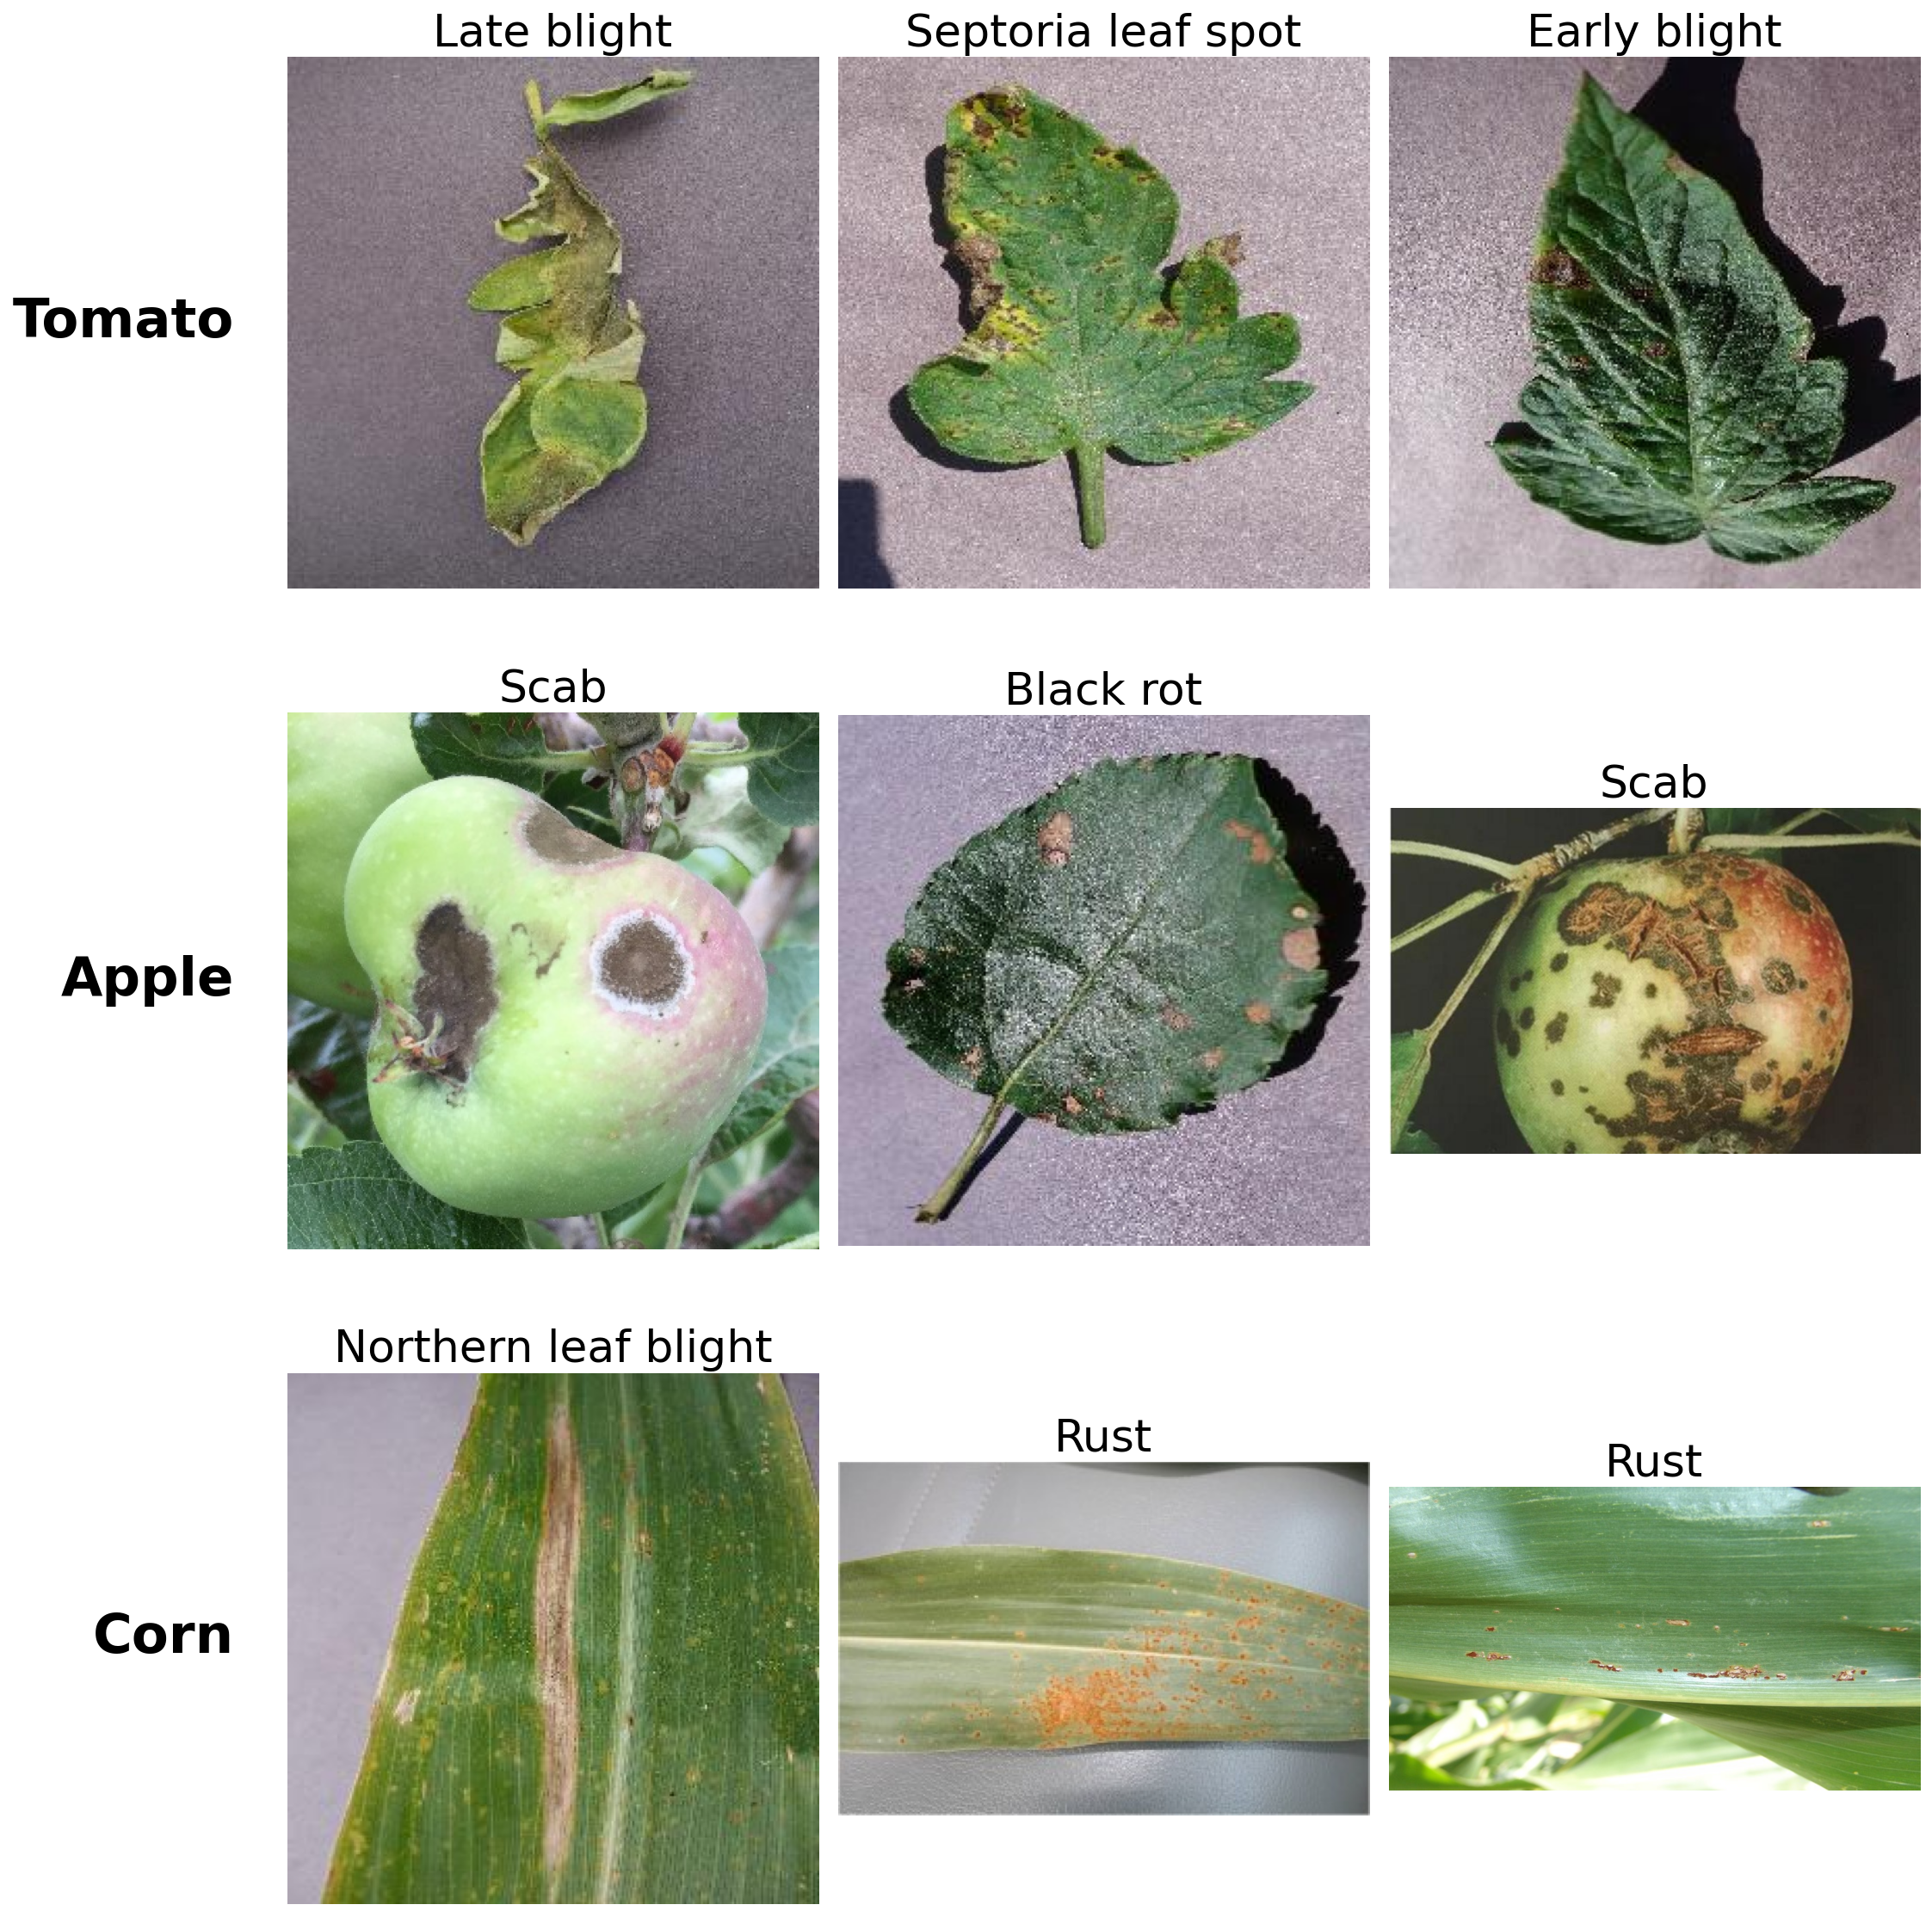
\includegraphics[width=0.6\columnwidth]{dataset_sample_grid.png}
  \caption{Samples from PlantWorld, showing diversity across crops (rows) and diseases (columns). This highlights the mix of `in-the-wild' images and lab-based images.}
  \label{fig:dataset_samples}
\end{figure}

\subsection{Dataset Statistics and Imbalance}

The distribution of images per crop is shown in Table~\ref{tab:dataset_dist}. The dataset is substantially imbalanced: Tomato contributes 20,455 images while Raspberry contributes only 620, a ratio of 33:1. This long-tail distribution reflects the underlying imbalance in publicly available agricultural imagery and motivates the imbalance-handling strategies described later.

\begin{table}
\begin{center}
\begin{tabular}{|l|c|l|c|}
\hline
Crop & Image Count & Crop & Image Count \\
\hline\hline
Apple       & 4027  & Potato    & 2774  \\
Banana      & 795   & Raspberry & 620   \\
Blueberry   & 1831  & Soybean   & 6181  \\
Cherry      & 2103  & Squash    & 2591  \\
Citrus      & 6030  & Strawberry& 1758  \\
Corn        & 5150  & Tomato    & 20455 \\
Grape       & 4781  & Wheat     & 1909  \\
Peach       & 3223  &           &       \\
Pepper bell & 2878  & Total     & 67166 \\
\hline
\end{tabular}
\end{center}
\caption{Image Count per Crop in the Unified Dataset.}
\label{tab:dataset_dist}
\end{table}

\subsection{Data Preprocessing and Enhancement}
Given the variety in image resolution, first we resize and center-crop every image to $224 \times 224$. The rationale for this dimension is that it is the standard input dimension accepted by the ViTs we elaborate on later.

After that, to prevent the model overfitting during training on the low-frequency cases, we augment the data using random flipping, rotations within 15 degrees, and color jitter; all these are possible cases when taking photos of crops in the field. This is applied both during training for crops and training for disease. Stratified splits were done after dataset aggregation to prevent data leakage.

% ---------------------------------------------------------------
\section{Reference Pipeline}
\label{sec:method}

\subsection{Crop Detection}

This is the first stage in our reference pipeline. We opted for ViTs, which have shown great success in other fields, but have seen limited application in crop and disease classification as noted by Thakur \etal~\cite{thakur2022plantvit}. Specifically, we selected MobileViT by Mehta and Rastegari~\cite{mehta2022}, a hybrid neural network that combines the efficiency and local inductive bias of CNNs with the global reasoning capabilities of transformers. This is critical to capture local patterns of crops, while maintaining the global context of the plant.

The variant selected was MobileViT-S -- pretrained on ImageNet-1k under 300 epochs -- which has 4.99M parameters; this is significantly smaller than ViT-Base, which has 86M parameters. Furthermore, MobileViT-S is more applicable towards edge computing while maintaining impressive accuracies as seen in examples like MobilePlantViT~\cite{tonmoy2025mobileplantvit}.

\subsection{Disease Detection}
For this model, there are two inputs: the image of the crop, and the label of the identified crop from the previous stage. Hence, this stage implements an architecture fusing visual features with semantic crop context predicted by the previous stage.

Our approach is to use a MobileViT-S as the backbone. Through this, we have a visual stream where we extract the global average-pooled feature representation (a 640-dim vector) from its final stage. Next, we have a learnable embedding layer, which maps the discrete crop ID to a dense 32-dim vector. Because of this, our model can learn latent relationships between different types of crops.

Finally, both vectors are fused to form a 672-dim state vector. We then perform layer normalization to stabilize the scale difference between the pre-trained ViT features and the embeddings trained on our dataset labels. This is followed by a multi-layer perceptron classifier with dropout(0.5) for regularization.


\subsection{Implementation Details}

\begin{figure}
    \centering
    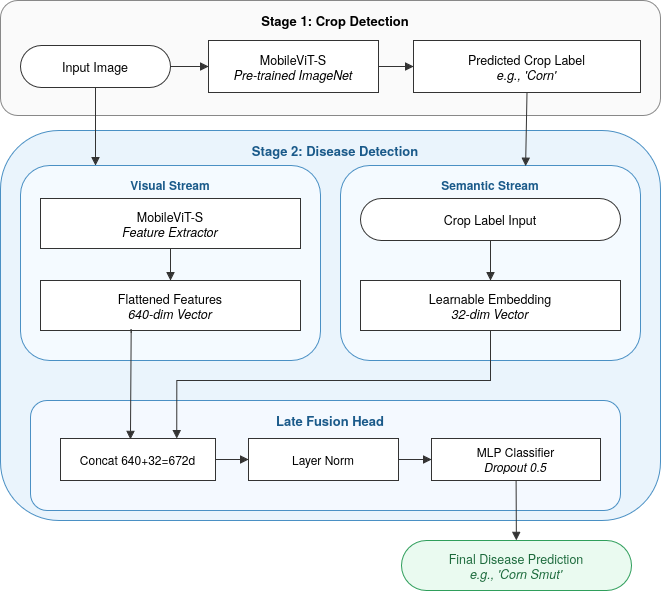
\includegraphics[width=0.75\linewidth]{architecture3.png}
    \caption{Overview of the two-stage architecture, demonstrating the fusion of crop predictions with visual features.}
    \label{fig:architecture}
\end{figure}

For the crop detection model, the loss function selected was weighted cross-entropy, to address the class imbalance in our dataset. Classes with fewer images get a higher weight, which is calculated as:
\begin{equation}
    w_c = \frac{1}{\sqrt{N_c}}
\end{equation}
where $N_c$ is the count of class $c$. This is done so that rare classes can receive appropriate representation. Moreover, we applied label smoothing with 0.1 for regularization (preventing overconfidence through slight adjustments of the target probability distribution). Our optimizer is AdamW~\cite{loshchilov2017decoupled}, a variant of Adam that implements weight decay (set to 0.01), and our learning rate is 0.0001 through empirical tuning. We also implemented a learning rate scheduler, particularly cosine annealing, so that the learning rate is adjusted to follow a cosine curve after each epoch, eventually approaching a minimum at the end of a cycle (we set 20 epochs) and hence encouraging better final convergence.

For the disease detection model, we retain the same implementation details; however, instead of weighted cross-entropy loss, we implemented focal loss ($\gamma=2.0$)~\cite{lin2017focal}. This is because our dataset contains significant class imbalance as well as visually similar phenotypes, which are significantly harder to classify, so this dynamic loss function down-weights well-classified examples -- such as healthy or distinct diseases -- and forces the model to focus on these misclassified examples. Furthermore, this model was trained separately from the previous stage.

\section{XAI Framework}

To investigate the factors driving the classifications of a model trained on this dataset, we also present an XAI framework that tests uncertainty, explainability, and robustness.

For uncertainty estimation, we introduce Monte Carlo Dropout at test time. This is grounded in its equivalence to approximate Bayesian posterior sampling~\cite{gal2016dropout}. In particular, we estimate the predictive entropy of the model by performing 25 stochastic forward passes, so that the model's confidence in its prediction can be quantitatively measured, improving reliability in the field.

As for model explainability, the industry standard is the use of Grad-CAM methods (to name a few, XGradCAM, ScoreCAM, FullGrad, and LayerCAM). However, as these were created mainly for CNNs, these are mostly gradient-based methods relying on backpropagation, and when applied to ViTs the heatmaps produced are much noisier and scattered due to blending of information from different tokens~\cite{abnar2020quantifying}.

We evaluated two methods: EigenCAM~\cite{bany2020}, which uses PCA of learned features and is class-agnostic, and GradCAM++~\cite{chattopadhay2018}, which uses class-discriminative gradient weighting. Through aggregate evaluation using the deletion metric (described below), GradCAM++ produced more faithful localization maps and was adopted as our method of choice.

For robustness, visual inspection of the heatmaps is not enough. We implemented three quantitative metrics:

\begin{itemize}
    \item Intensity analysis using feature ablation, where we assign weights to each input type (visual and semantic). The image is masked and the model's drop in confidence is measured; the same is done with the crop label independently. The percentage split is then normalized, quantifying what the model prioritizes (e.g. $77\%$ visual vs $23\%$ semantic for clean laboratory images).

    \item Counterfactual testing, where the wrong crop label is provided (for example, giving "Banana" instead of "Corn") and the prediction is observed. If visual evidence is dominant, the model is expected to retain the correct prediction.

    \item Deletion metric and Area Under Curve (AUC). The most important pixels identified by GradCAM++ are iteratively removed, and the model's drop in confidence is tracked. A low AUC signals that the highlighted pixels were genuinely driving the decision thus confirming a causal relationship~\cite{petsiuk2018rise}.
\end{itemize}

% ---------------------------------------------------------------
\section{Results and Discussion}
\label{sec:results}

\subsection{Crop Detection Results}

We trained our model with a stored stratified dataset split of 70\% for training, 15\% for validation, and 15\% for testing. Our final training accuracy was 98.89\% which corresponds to almost perfect classification of crops. Validation accuracy was similar to this at 97.6\%, which meant that our model was almost certainly generalizing well on the dataset. The performance of the model converged in only 5 epochs.

The model was then tested on the test split, which yielded a final top-1 accuracy of 98.48\% with a loss of 0.6293; considering the sheer size and complexity of our dataset, this is strong performance. When considering how the model treats different classes, the weighted-averaged F1-score reported by our model is 98.87\%, so our modifications to optimization and regularization were successful.

\begin{figure}[h]
  \centering
  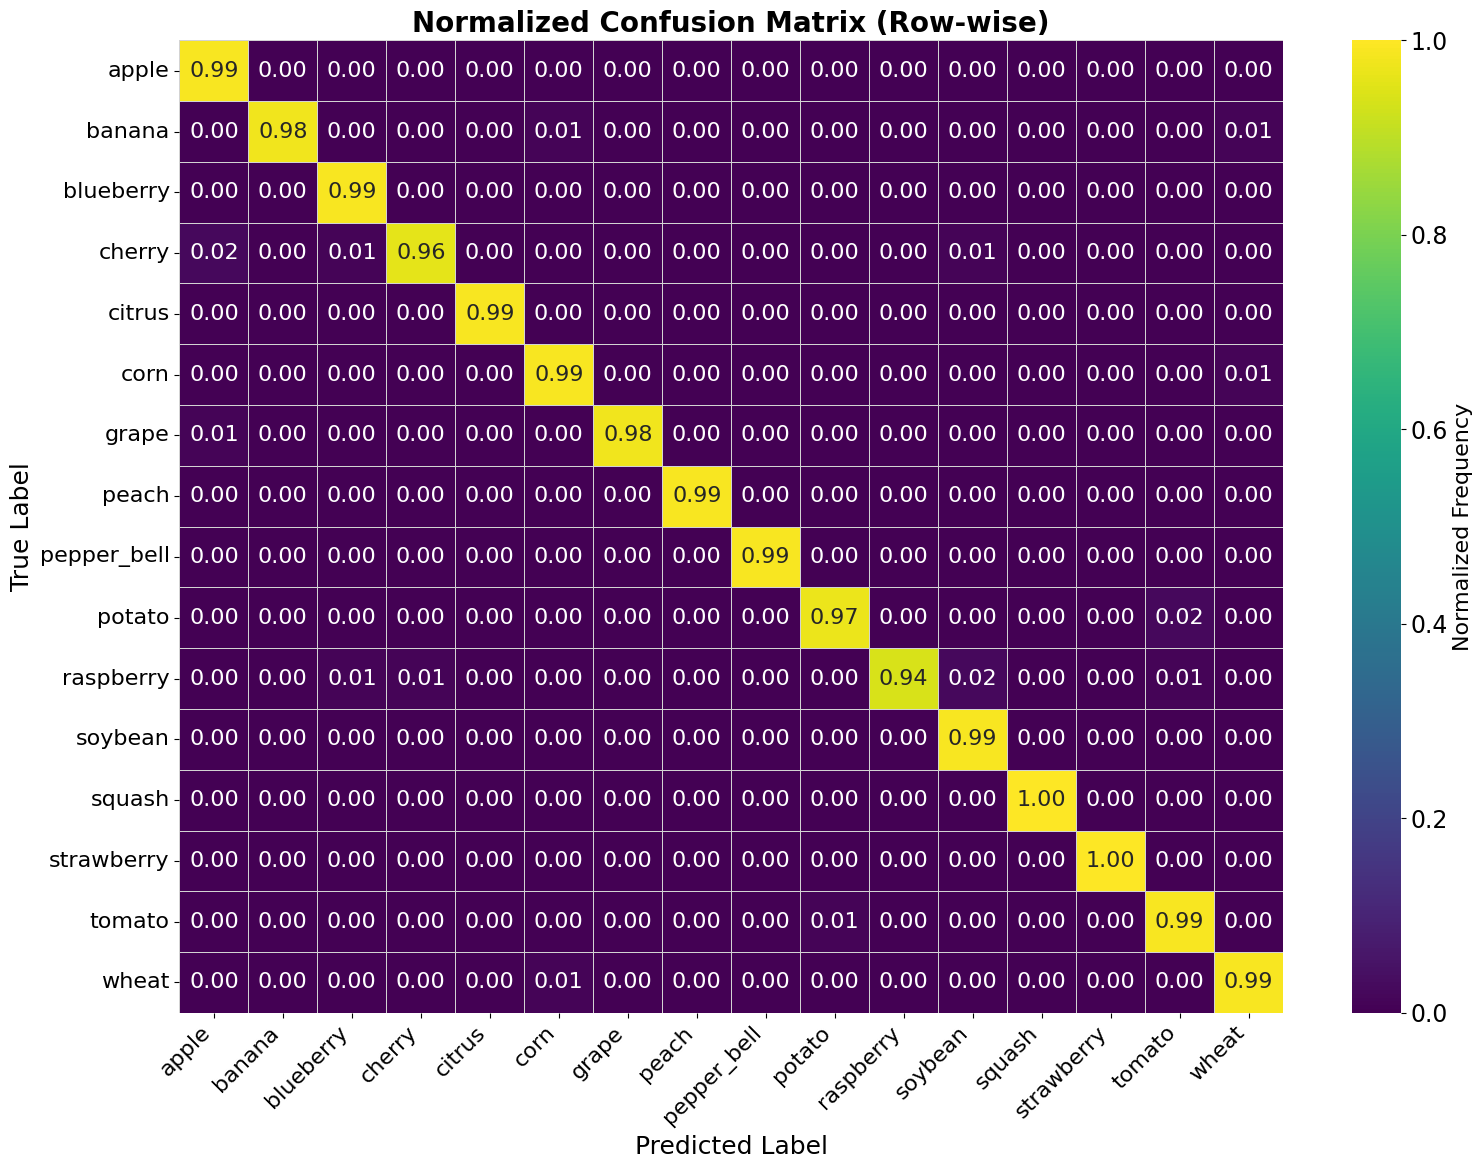
\includegraphics[width=0.9\columnwidth]{Screenshot_20251209_222538.png}
  \caption{Confusion matrix for crop detection.}
  \label{fig:crop_cm}
\end{figure}

\subsection{Disease Detection Results}

The disease detection was also successful. The model showed high generalization on the test set, with a final test accuracy of $96.62\%$ and a test loss of $0.0496$, which is competitive with figures presented by literature for disease classifiers of single crops. The model converged in 16 epochs, with divergence occurring thereafter in test loss, so early stopping was triggered.

\begin{figure}[h]
    \centering
    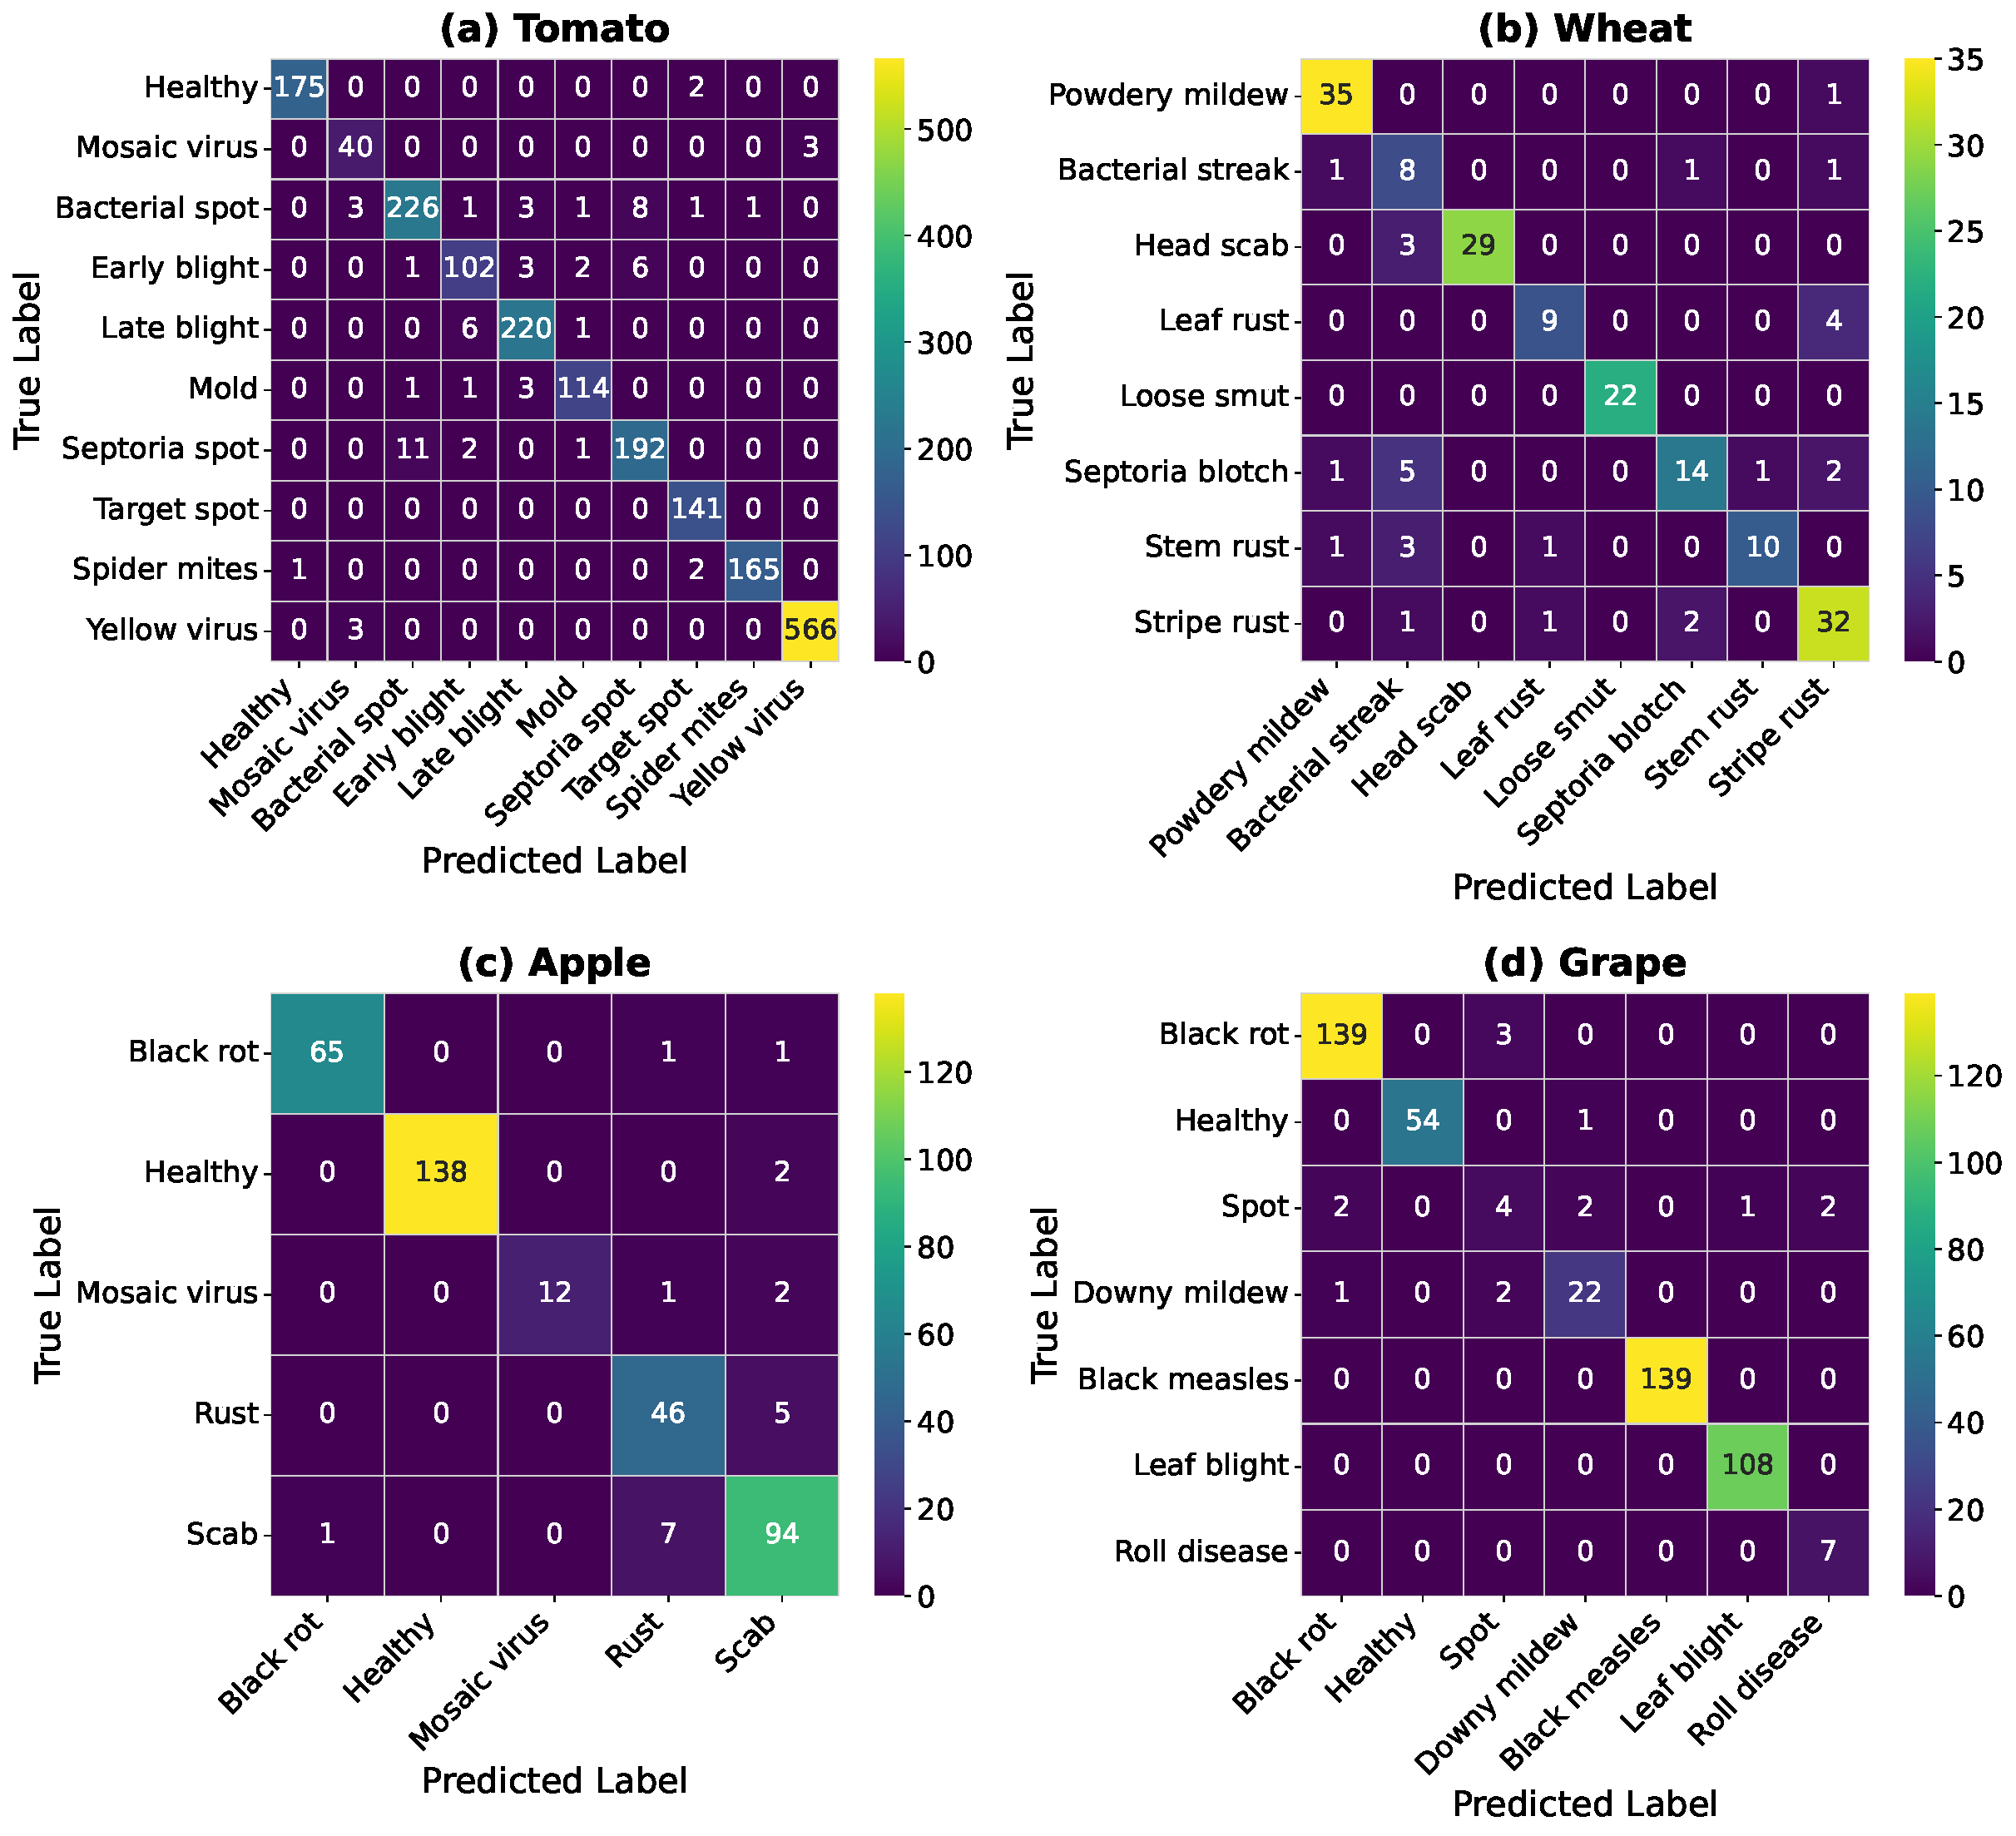
\includegraphics[width=0.9\textwidth]{disease_matrices.pdf}
    \caption{Confusion matrices of four crops: Tomato, Wheat, Apple, and Grape.}
    \label{fig:dismat}
\end{figure}

During testing, we were interested in the robustness of the model across the biological domains of the crops. Hence, the confusion matrices of the four most populous crops were generated as seen in~\ref{fig:dismat}. Strong diagonal dominance is observed in all four matrices, with the predicted label matching generally with the true label. The few instances of off-diagonal elements were noted to be due to visually similar diseases within a single crop (e.g. "early blight" versus "late blight"), not because of model confusion over disparate conditions.

To validate the contribution of the crop embedding in Stage 2, we trained an image-only baseline using an identical MobileViT-S backbone and classifier but without the learnable crop embedding, operating on the same 54 disease classes. The image-only baseline achieved $94.90\%$ test accuracy compared to $96.62\%$ for the fusion model, a drop of $1.72$ percentage points attributable solely to excluding the crop embedding. Hence, the semantic crop prior provides meaningful information which is not otherwise present in the visual features, particularly for shared disease conditions such as {\em early\_blight} which manifest similarly across crops but benefit from knowing which crop is under inspection. Moreover, we also noted that the fusion model converged at epoch 17, while the baseline needed till epoch 20, so the crop embedding may also be simplifying optimization.

\subsection{Two-Stage Pipeline Results}

We connected the two trained models together in one pipeline which, given an image, identifies its crop and uses the crop label embedding to identify its disease, if any. This was tested on our usual test dataset split of 6571 samples. The results are as follows: overall accuracy ended at $95.77\%$ with stage 1 crop accuracy at $98.48\%$. Notably, for the samples where the crop label was predicted correctly, disease accuracy was $96.82\%$, whereas for the remaining 100 ($1.5\%$) samples with incorrect crop label prediction, the disease accuracy plummeted to $28.00\%$. This implies that stage 2's performance is heavily reliant on stage 1's performance.

Moreover, since the major use case of this system is deployment in budget smartphones owned by farmers, we applied Post-Training Dynamic Quantization to convert 32-bit floating point weights to 8-bit integers to reduce the model size while retaining accuracy. This reduced overall pipeline size from 21MB to 11MB (45\% reduction) along with a negligible +0.07\% accuracy change due to noise; thus, this quantization indicates the possibility of deployment on edge devices.

\subsection{Explainability and Robustness Analysis}

With Monte Carlo Dropout, we stratified test predictions by estimating the entropy from the stochastic passes; if the entropy is below 0.5, we defined it to be a confident prediction. Our analysis revealed that 81\% of the test data was flagged as confident, where the model achieved 99.92\% accuracy. The remaining 19\% images were correctly flagged as uncertain, with a respective accuracy of 82.47\%; hence, in deployment, the system could defer these cases to human experts.

To test XAI capabilities, we evaluated both EigenCAM and GradCAM++ for heatmap generation and adopted GradCAM++ as it produced more class-discriminative maps, confirmed by lower deletion AUC scores across our aggregate evaluation. Figure~\ref{fig:top5_heatmaps} shows the five most faithful heatmaps from the diseased images of our test set (since the healthy images do not involve lesion localization), selected by lowest deletion AUC. In most cases, the heatmaps show the model focusing on the crop leaves (with the exception of the bottom right corner of image 4). Since the AUC is extremely low, the prediction likely depends on not just the diseased lesion but a large area surrounding it, which warrants further investigation.


\begin{figure*}[h]
    \centering
    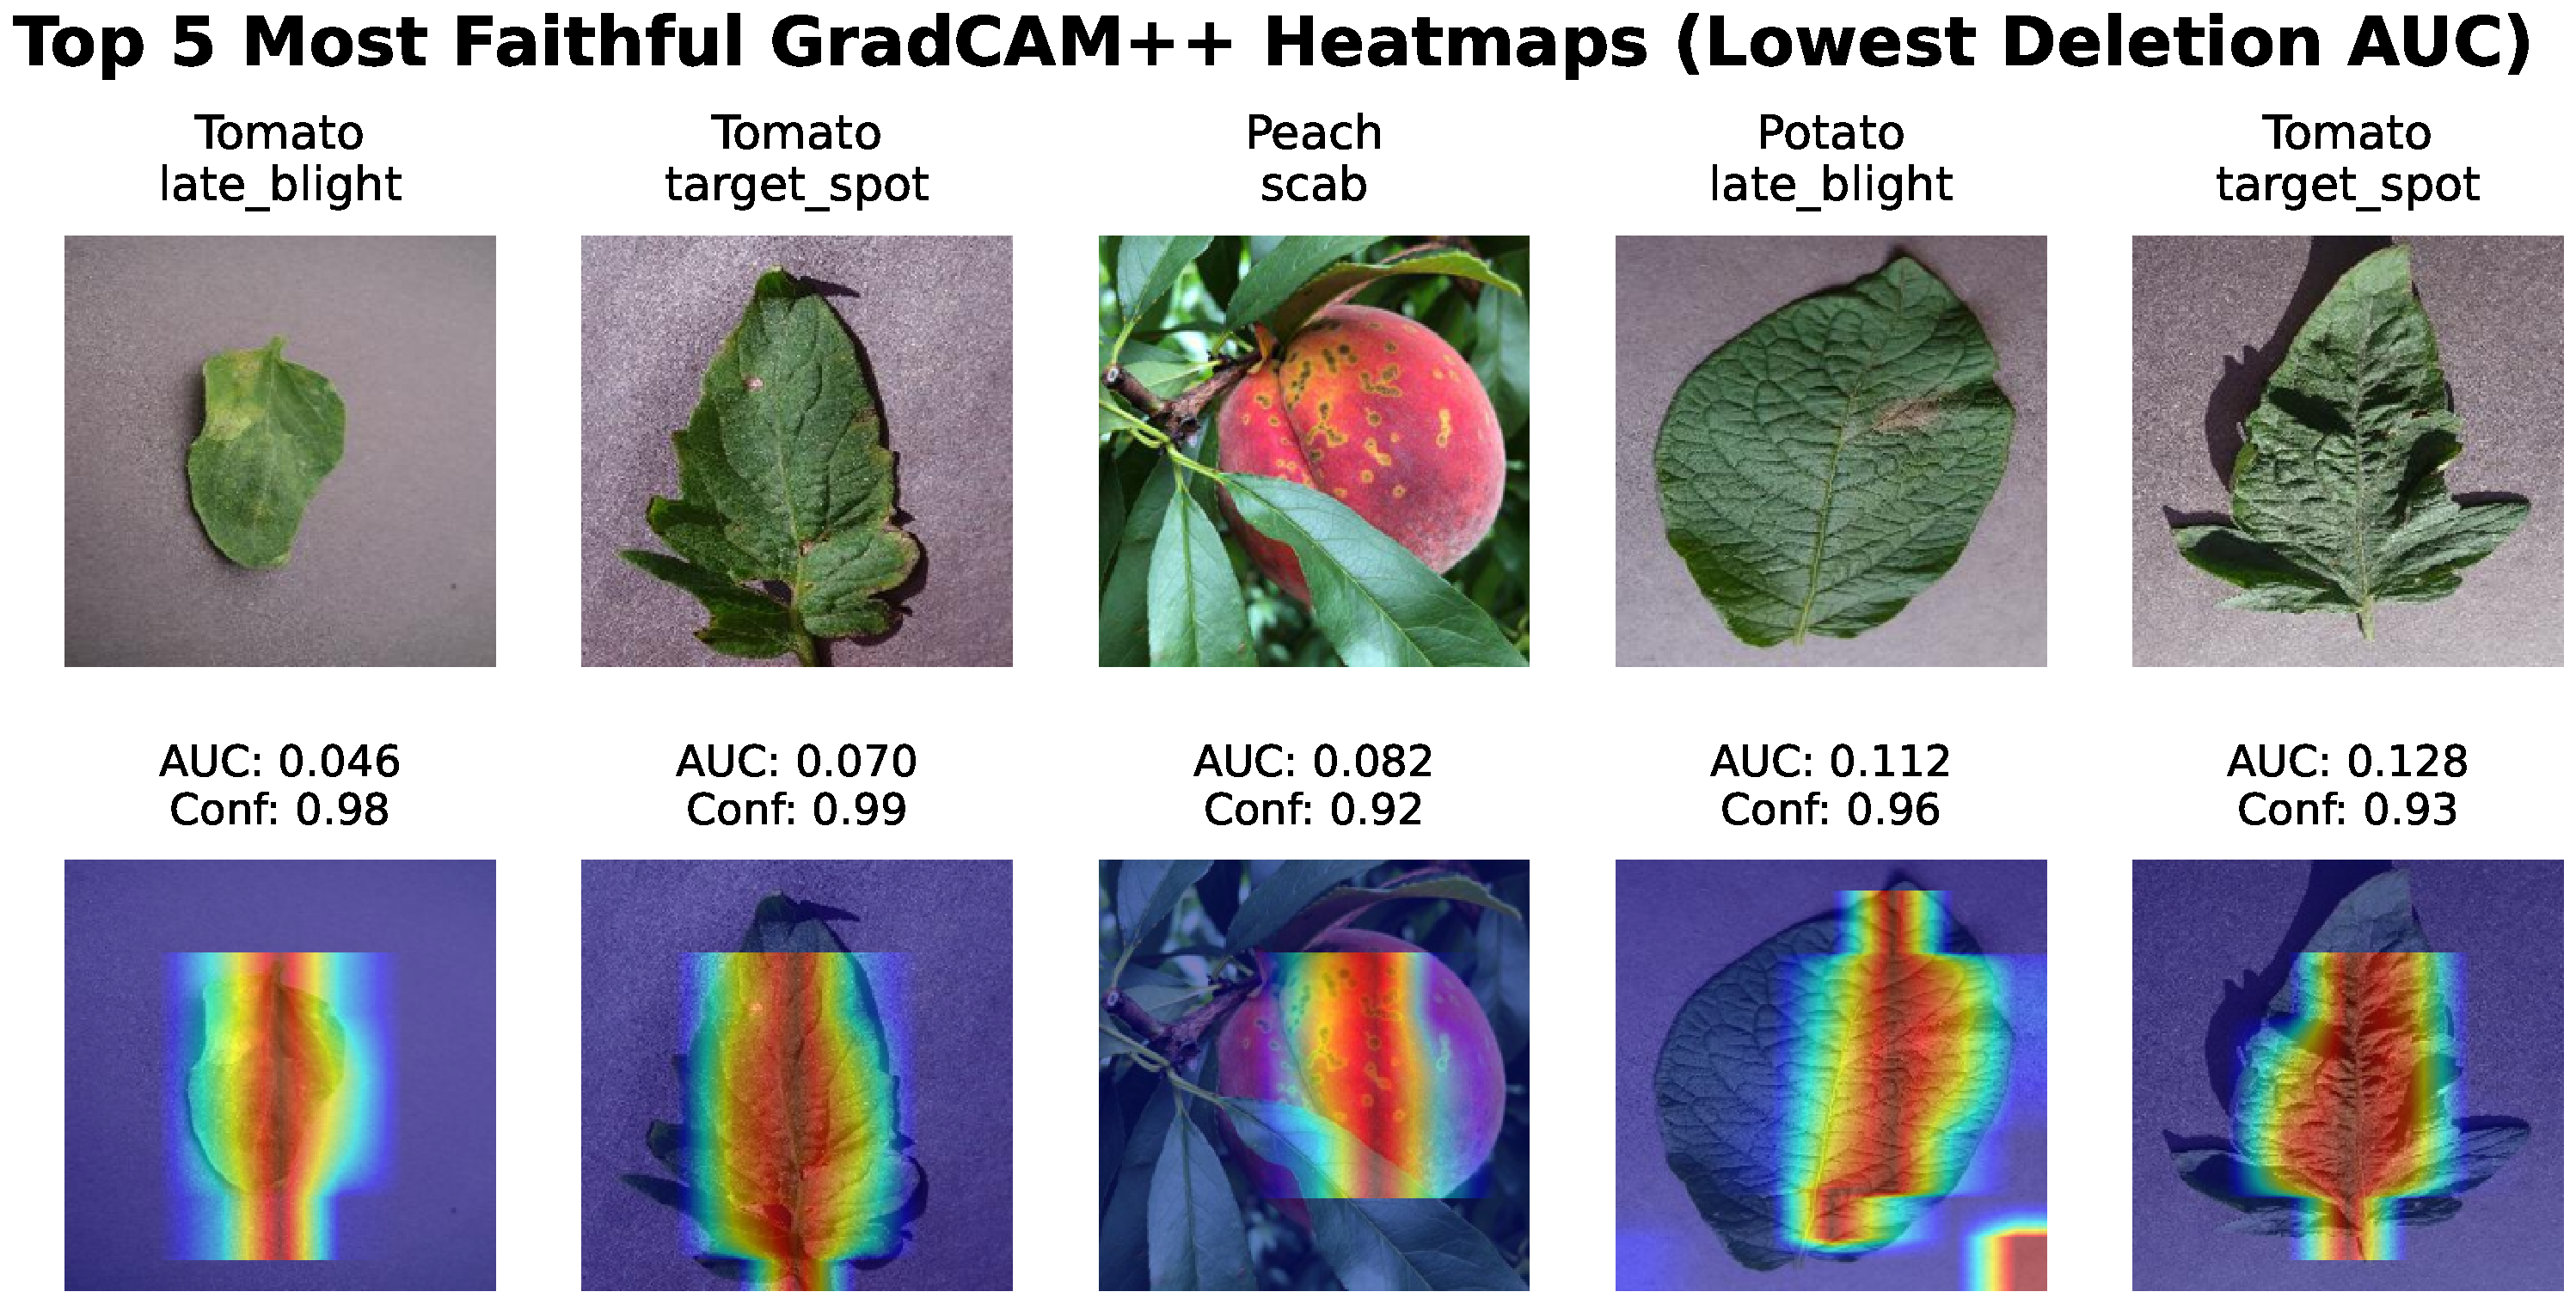
\includegraphics[width=0.9\textwidth]{images/fig_top5_heatmaps.pdf}
    \caption{Top row: original images. Bottom row: GradCAM++ overlays with deletion AUC and confidence scores.}
    \label{fig:top5_heatmaps}
\end{figure*}

To validate XAI behaviour beyond individual examples, we conducted an aggregate analysis over a per-crop stratified sample of 678 test images across all 16 crops. We generated GradCAM++ heatmaps for each sample and computed the corresponding deletion AUC, intensity split, and counterfactual testing.

The aggregate deletion AUC was $0.521 \pm 0.218$, which was a substantial improvement over EigenCAM ($0.683 \pm 0.190$); this confirms that GradCAM++ produces more faithful localization for our use case. The per-crop breakdown in~\ref{fig:deletion_auc_per_crop} reveals a biologically coherent pattern: crops with focal lesions such as tomato ($0.362$) and soybean ($0.405$) achieved the lowest AUC scores, so the model's decisions are concentrated on pathological regions. On the other hand, crops such as citrus ($0.689$) and strawberry ($0.678$) showed higher AUC, because their disease signals are distributed across the entire leaf surface.

\begin{figure}
    \centering
    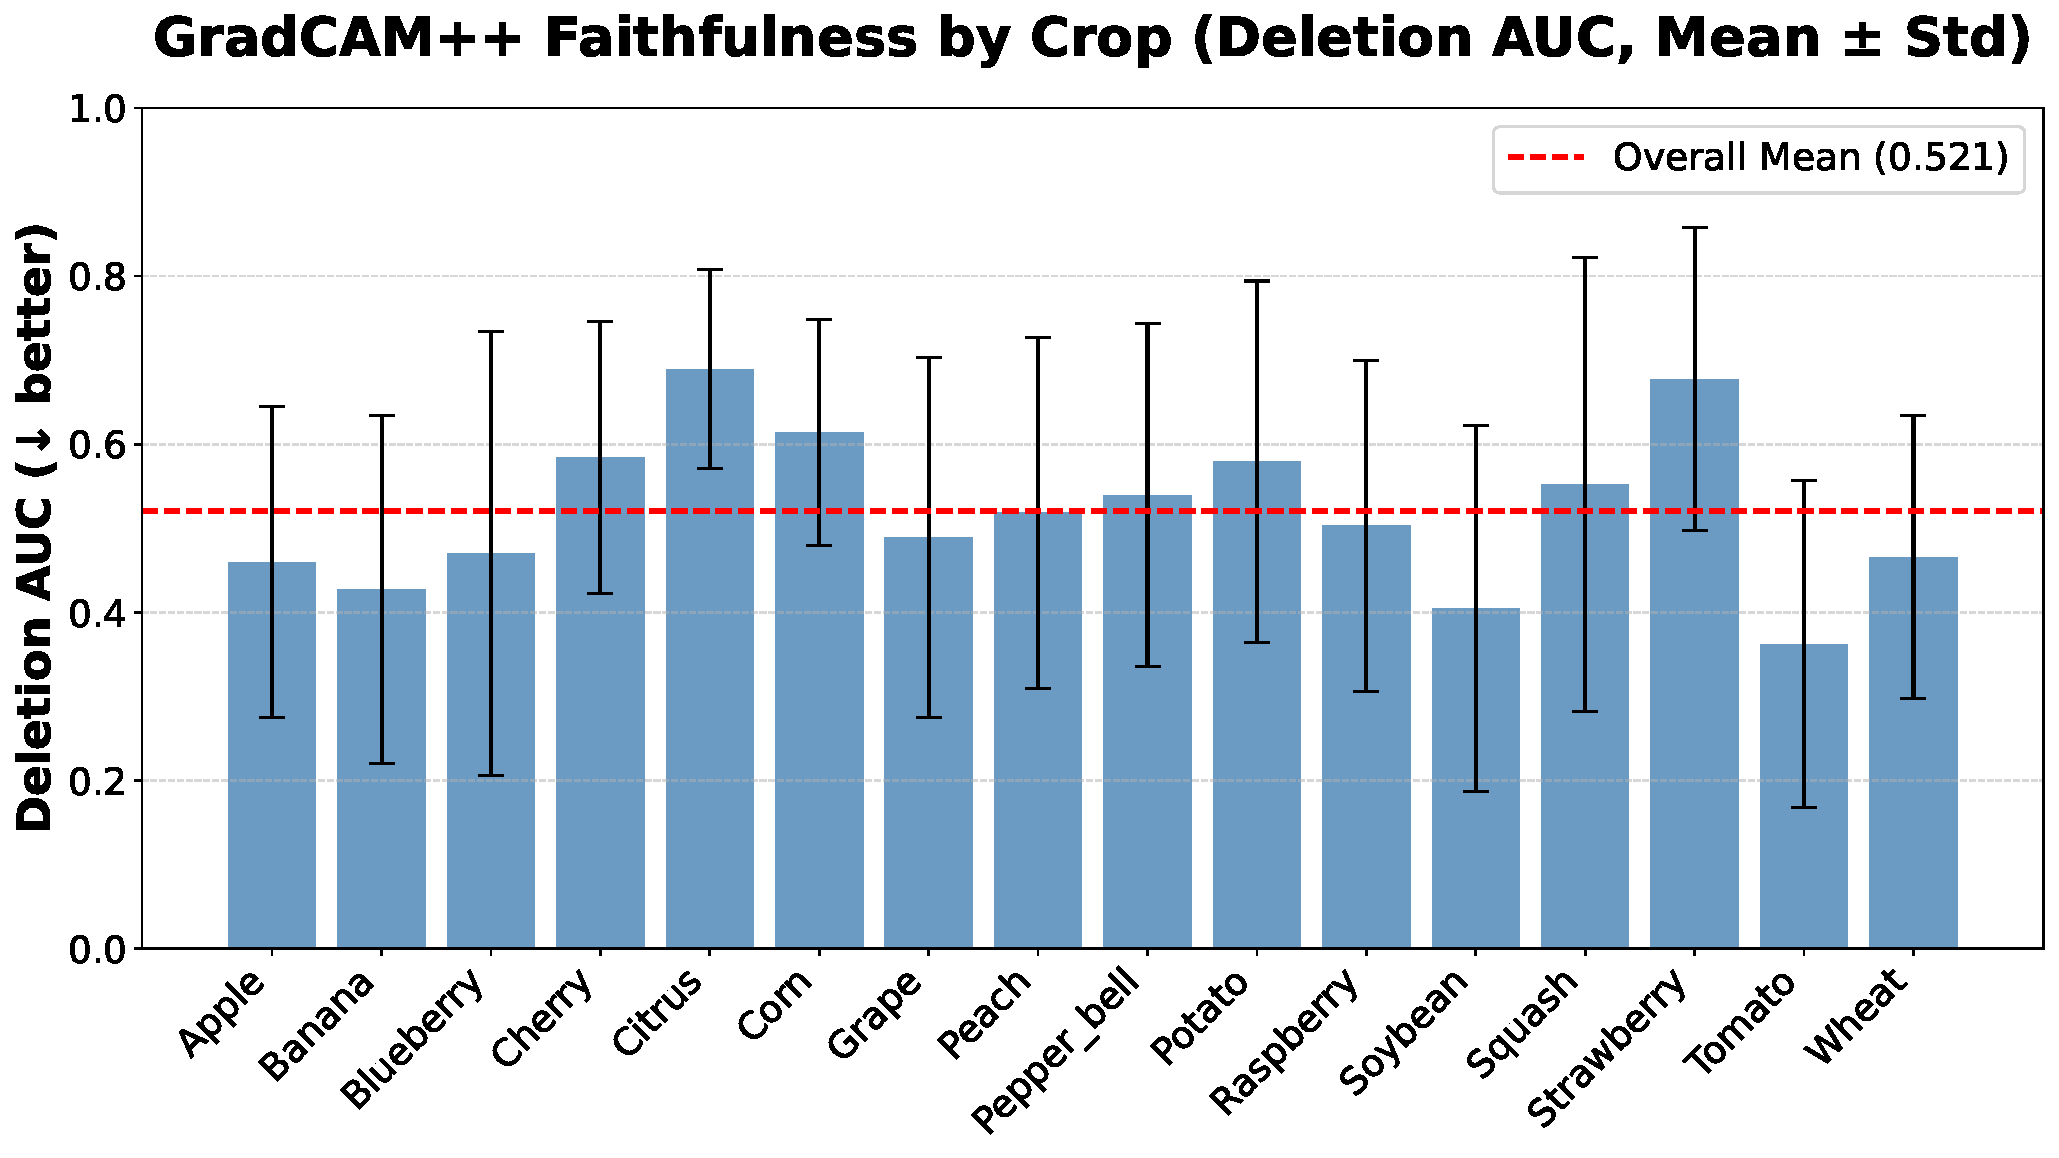
\includegraphics[width=0.7\linewidth]{fig_deletion_auc_per_crop.pdf}
    \caption{Per-crop deletion AUC for GradCAM++ heatmaps across 678 test samples.}
    \label{fig:deletion_auc_per_crop}
\end{figure}

Intensity analysis across all samples returned a mean attribution split of $62.4\%$ visual and $37.6\%$ semantic. When stratifying by image source (\ref{tab:intensity_source}), we see that this figure is dependent on dataset composition: PlantVillage and PlantDoc images show high reliance on vision ($77.4\%$ and $77.0\%$), while PlantWild images shift to $46.4\%$, indicating the model gives high importance to the label as a prior when visual evidence is ambiguous under real-world conditions.

\begin{table}
\centering
\caption{Intensity split and deletion AUC by image source.}
\label{tab:intensity_source}
\begin{tabular}{lccc}
\hline
\textbf{Source} & \textbf{n} & \textbf{Visual \%} & \textbf{AUC} \\
\hline
PlantVillage & 324 & $77.4 \pm 19.2$ & $0.574 \pm 0.214$ \\
PlantDoc     & 26  & $77.0 \pm 23.5$ & $0.571 \pm 0.200$ \\
PlantWild    & 328 & $46.4 \pm 20.2$ & $0.464 \pm 0.208$ \\
\hline
\end{tabular}
\end{table}

The per-crop intensity breakdown in \ref{fig:intensity_split} further demonstrates which crops drive semantic reliance. Citrus ($65.8\%$ semantic) and banana ($57.0\%$) show the highest semantic dependence, both of which are predominantly PlantWild-sourced crops with visually complex field backgrounds. In contrast, tomato ($23.5\%$ semantic) and potato ($22.8\%$) are visually dominant, consistent with their large PlantVillage representation and distinct lesion patterns. Apple is a notable outlier at $100\%$ visual attribution, as it is nearly exclusively from PlantVillage where clean backgrounds leave no ambiguity to resolve.

\begin{figure}
    \centering
    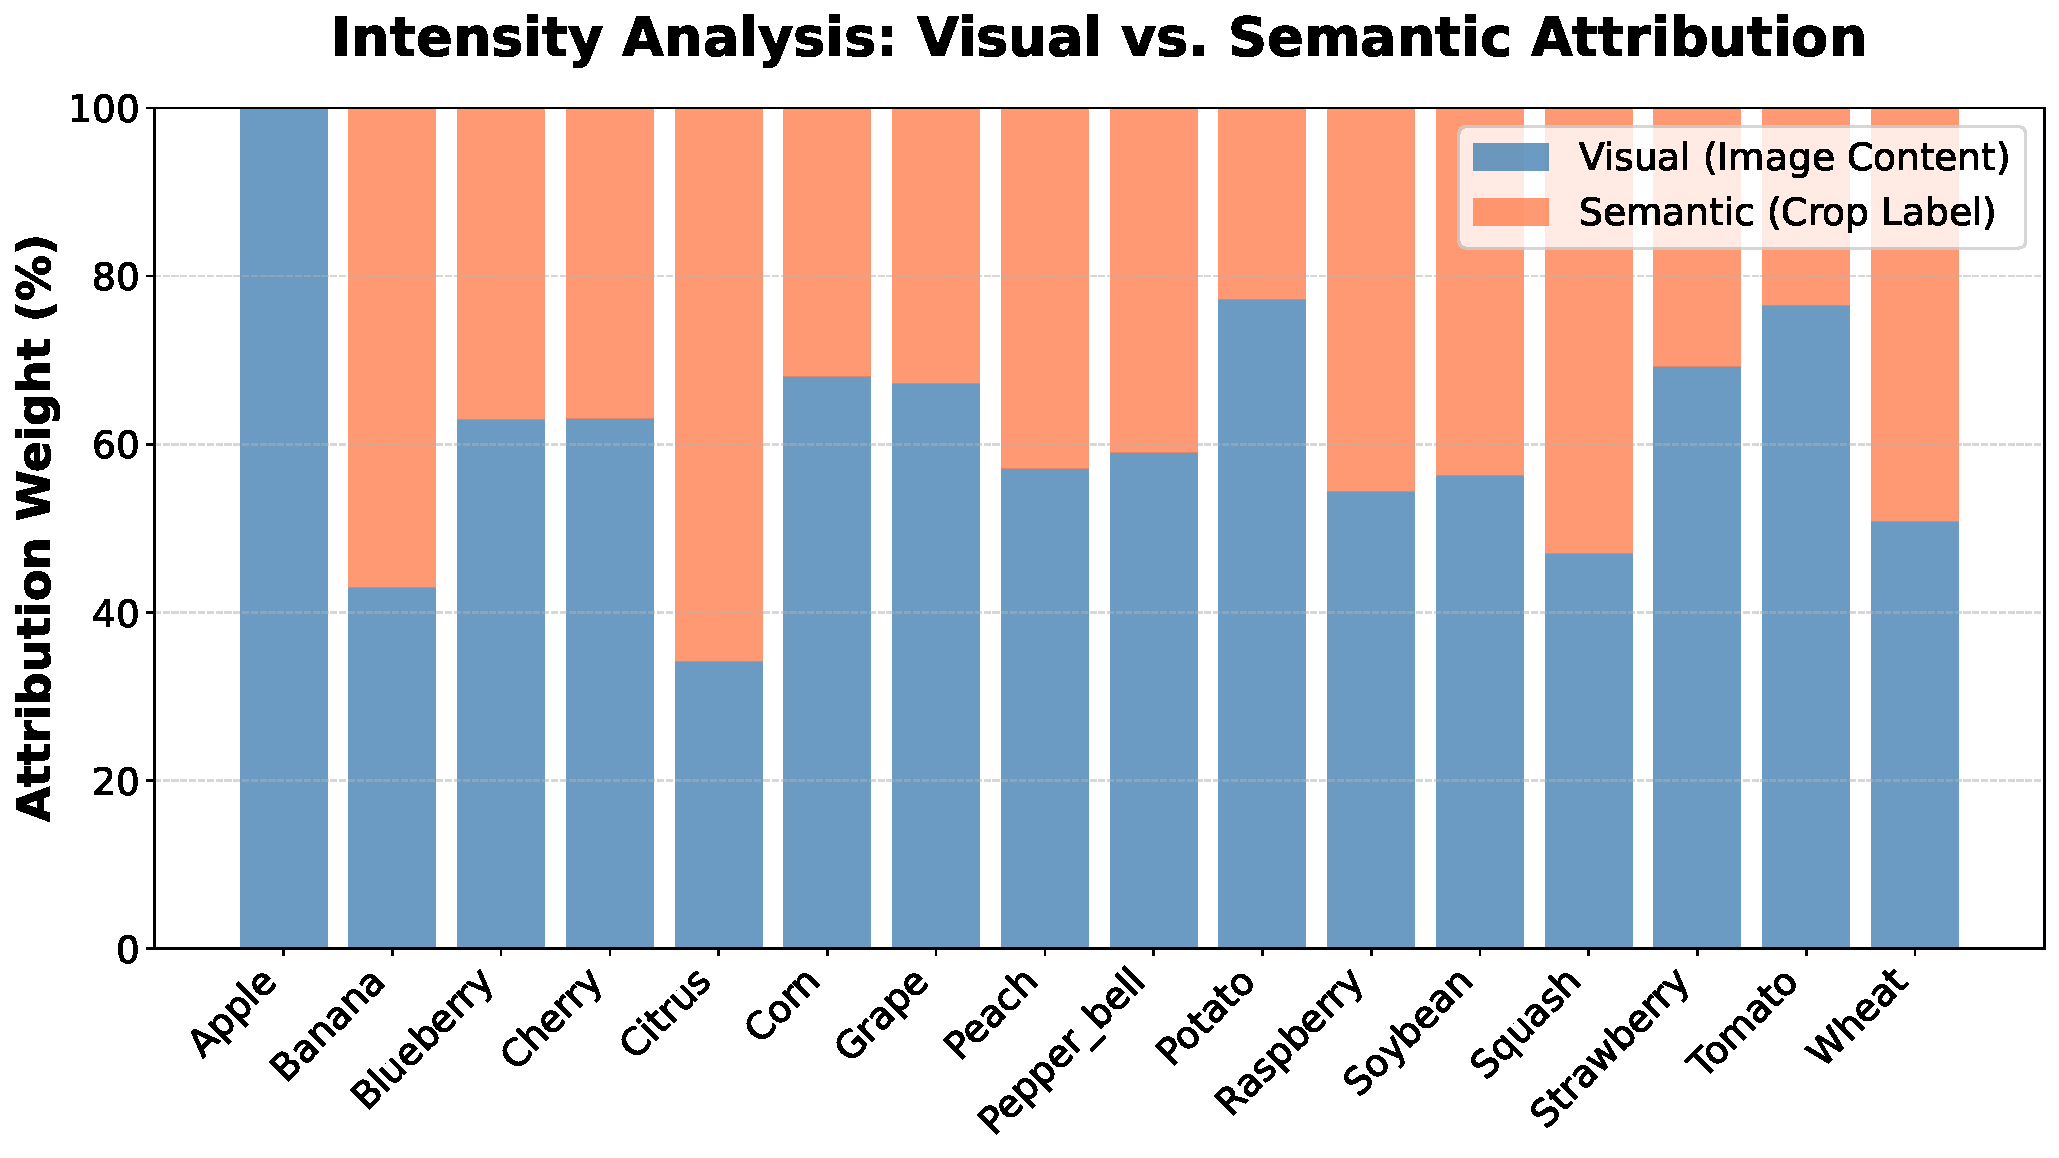
\includegraphics[width=0.7\linewidth]{fig_intensity_split.pdf}
    \caption{Per-crop visual vs.\ semantic attribution split. Crops with high semantic reliance (citrus, banana, squash, wheat) are predominantly sourced from in-the-wild datasets; visually dominant crops (tomato, potato, apple) are largely PlantVillage-sourced.}
    \label{fig:intensity_split}
\end{figure}

Counterfactual robustness testing (in which a wrong crop label was deliberately substituted) yielded a rate of $61.2\%$ -- that is, in $61.2\%$ of tests the model either retained the exact prediction or predicted a disease that is valid for the correct crop. This suggests that visual features remain the dominant signal for the majority of samples, though the model is not fully robust to incorrect semantic inputs, particularly for in-the-wild imagery.


\subsection{Comparison with Methods}

As our dataset is new, comparison with current literature is unfair since they were trained and tested on different datasets. Hence, we selected multiple models that have had historically excellent performance in plant disease classification~\cite{shafay2025recent, pal2025lightweight} while including similar models for image classification allowing us to explore this task beyond literature. For reference, these models directly predict crop and disease in one go, which we accomplished on a flattened version of our dataset where each label is a combination of crop and disease, thus resulting in 86 crop-disease combinations. Our results are showcased in Table~\ref{tab:wild_comparison}.

Among higher capacity models, ConvNeXtV2-Tiny, DeiT-Small and ViT-Small achieve the highest accuracy around $96.7\%$. However, their numbers of parameters require at least double that of the reference pipeline, even if still small enough to be deployed. The established CNN baselines (ResNet-50 and EfficientNet-B4) are outperformed by the transformer-based models. There is also a noticeable cluster at 95.60-95.75\% comprising of Swin-Tiny, FastViT-SA24, LeViT-256, and PVT-v2-B1, even though the parameters span from as low as 13.54M to over double at 27.59M, which indicates that parameter count may not predict accuracy well. In particular, Swin-Tiny is outperformed even by the reference pipeline, which is far lighter. However, the pipeline's cascading dependency is a tradeoff against the more accurate but heavier models and the lighter but less accurate models.

Overall, this table establishes reference points for future work on PlantWorld, so that new models can be benchmarked against these results, both on accuracy and parameter count.

\begin{table}
\centering
\caption{Comparison of plant disease detection architectures on our unified benchmark dataset, sorted by parameter count.}
\label{tab:wild_comparison}
\begin{tabular}{|l|c|c|}
\hline
\textbf{Method} & \textbf{Params} & \textbf{Acc. (\%)} \\
\hline\hline
ConvNeXtV2-Tiny~\cite{woo2023convnext} & 27.93M & 96.62 \\
Swin-Tiny~\cite{liu2021swin} & 27.59M & 95.60 \\
ResNet-50~\cite{he2016deep} & 23.68M & 94.63 \\
DeiT-Small~\cite{touvron2021training} & 21.70M & 96.77 \\
ViT-Small~\cite{dosovitskiy2020image} & 21.70M & 96.67 \\
FastViT-SA24~\cite{vasu2023fastvit} & 20.62M & 95.75 \\
LeViT-256~\cite{graham2021levit} & 17.96M & 95.75 \\
EfficientNet-B4~\cite{tan2019efficientnet} & 17.70M & 94.28 \\
PVT-v2-B1~\cite{wang2022pvt} & 13.54M & 95.60 \\
MobileViT-S~\cite{mehta2022} & 4.99M & 94.76 \\
\hline
Reference (2x MobileViT-S) & 9.98M & 95.77 \\
\hline
\end{tabular}
\end{table}

\section{Conclusion and Future Directions}
\label{sec:conclusion}

In this paper, we have presented PlantWorld as a unification of foundational datasets for crop and disease identification, with taxonomic harmonization. We also provide an XAI framework, leveraging Monte Carlo Dropout for uncertainty, GradCAM++ for heatmaps, intensity analysis for feature attribution, counterfactual testing, and deletion AUC for robustness. Through this, we can investigate whether a model focuses on the correct portions of the image, instead of background noise, which offers potential as a useful tool for precision agriculture. We have also benchmarked multiple models, including a reference pipeline as a baseline for comparison. We recommend PlantWorld and its benchmark for future models in this domain.

\subsection{Limitations}

The reference pipeline has limitations, which we discuss here.

\begin{itemize}
    \item Confusion matrices show that the model struggles to differentiate between visually similar phenotypes, such as "Early Blight" and "Late Blight" in the "Tomato" class. This is likely due to the global attention mechanism inherent in the ViT backbone; while this is effective for structure, this can cause the model to miss small details that separate such similar necrotic patterns.
    \item The nature of the architecture carries a risk of cascading error dependency. If the first stage misclassifies the crop, the second stage is more likely to provide an incorrect diagnosis, especially when visual evidence is unclear. This is quantitatively supported by our counterfactual robustness analysis, which found that 61.2\% of predictions retain under a wrong crop label, while the remaining 38.8\% flip; this worsens for in-the-wild imagery where the model relies more heavily on the semantic prior.
    \item Due to the nature of the pipeline, uncertainty can propagate down the stages. The XAI framework presented does not account for this situation.
\end{itemize}

\subsection{Future Directions}

We offer avenues for exploration to resolve the limitations.
\begin{itemize}
\item A method to mitigate confusion between visually similar diseases is supervised contrastive learning (SupCon), which encourages the model to utilize label information to learn more effectively~\cite{khosla2020supervised}.
\item The late fusion method can be swapped out for the more sophisticated cross-attention mechanisms, where the semantic crop embeddings can query visual features within the transformer layers directly instead of being concatenated. This way, visual attention on the crop type can happen earlier in the process, informing a potentially better decision while also potentially reducing complexity as demonstrated by Chen \etal~\cite{Chen_2021_ICCV}.
\item We did not report inference latency of the models on edge devices. Since the typical use case is deployment on a budget smartphone, future models should benchmark latency on representative hardware to address this metric.
\end{itemize}

\bibliography{main}
\end{document}
